\section{Tree Structure CPDs}\label{sec:treeCPD}
Table CPDs are problematic when there are many many parents for a conditional variable.
Tree structure CPDs can handle a large set of parents given that there is certain \underline{context} provided.
\begin{marginfigure}
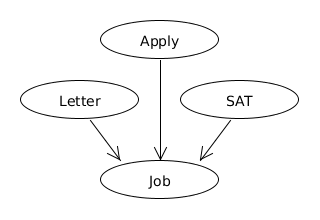
\includegraphics{images/100_01}
\caption{A simple CPD with four parents}
\label{fig:100_01}
\end{marginfigure}

\begin{marginfigure}
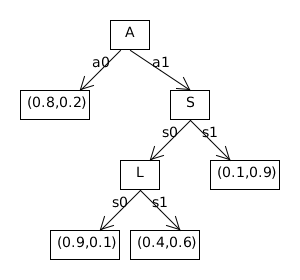
\includegraphics{images/100_02}
\caption{Tree based CPD for Figure~\ref{fig:100_01}}
\label{fig:100_02}
\end{marginfigure}


We start from the root and traverse the branches.  Each branch represents a CPD for a given set of conditions.  For example if a student does not apply for a job ($A=a^0$), then the probability of the student getting a job ($J=j^1$) is
\begin{itemize}
\item $P(j^1 | 	A,S,L)=0.2$
\item the probability is independent of $S,L$
\end{itemize}

